% !TeX root = main.tex
\section{Discussion}

Traditional collision-detection frameworks treat rendering as a
consumer of simulation state. In contrast, the gPCD framework
integrates occupancy generation directly into the graphics pipeline,
allowing occupancy construction and rendering to proceed concurrently.
The significance of this organization is architectural rather than
algorithmic. The framework does not introduce a new spatial data
structure; instead, it introduces a new execution model in which
graphics-pipeline operations contribute directly to broad-phase
collision detection.

An additional benefit of this organization is that synchronization is
largely confined to occupancy generation. Atomic operations are
required only when reserving slots within shared cell lists, while
subsequent collision discovery remains source-owned and proceeds
without construction of a globally shared collision-pair structure.
This organization maps naturally onto massively parallel GPU
architectures.

The throughput, time-per-particle, scaling, and curvature analyses are
all consistent with the theoretical \(O(N)\) occupancy-generation
behavior developed in the complexity analysis. Although
implementation-specific effects influence absolute execution times, the
measured scaling exponents remain close to unity and the corresponding
curvature bounds remain small, indicating that no dominant super-linear
behavior emerged over the evaluated benchmark range.

The measured scaling exponents remain close to unity and the
corresponding curvature bounds remain small, suggesting that no stage
of the framework introduces substantial nonlinear growth as particle
count increases.

Although throughput decreases within the throughput-transition regime
and the stable large-scale regime, the observed behavior remains
consistent with increasing resource utilization rather than a breakdown
of the underlying scaling characteristics of the framework.

The locality benchmark demonstrates that memory organization affects
performance independently of algorithmic complexity. Although
sequential and random occupancy layouts retain the same asymptotic
complexity, the increasing execution-time difference observed between
the two configurations indicates a measurable performance benefit from
improved memory locality.

The approximately parallel trends observed in
Figure~\ref{fig:A_PQBS_V_PQBR} suggest that memory locality primarily
affects implementation efficiency through memory-access costs rather
than the asymptotic scaling characteristics of the framework.


\begingroup
\begin{figure*}[ht]
\centering
\setlength{\fboxrule}{1pt}
\setlength{\fboxsep}{0pt}
\hspace{-0.1in}
	\begin{subfigure}[b]{0.3\textwidth}
		{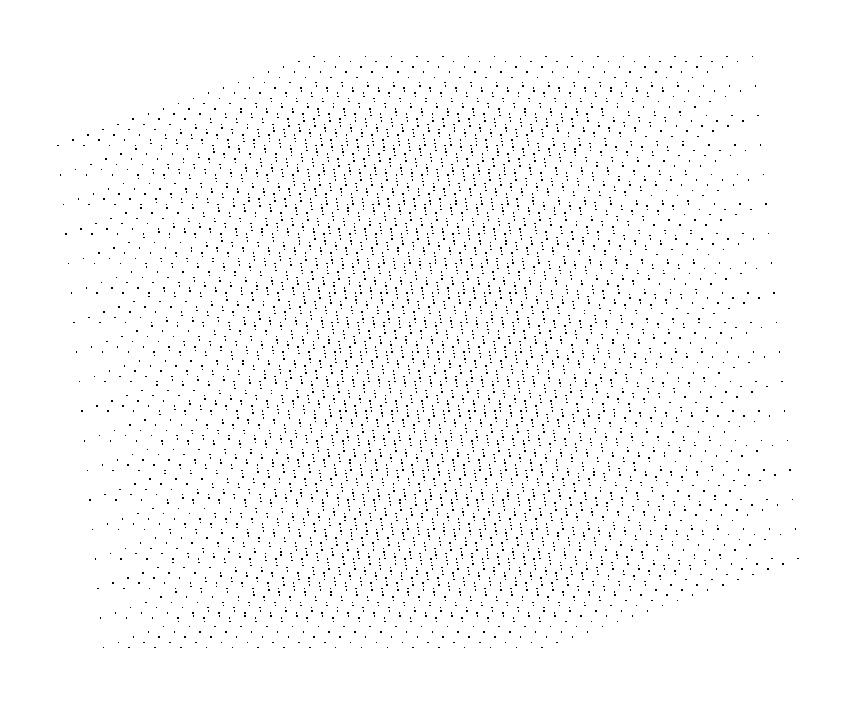
\includegraphics[width=\textwidth]{p5832.pdf}}
		\subcaption[]{5,832 particles (6000 fps)}
		\label{fig:p5832}
	\end{subfigure}
\hspace{-0.1in}
	\begin{subfigure}[b]{0.3\textwidth}
		{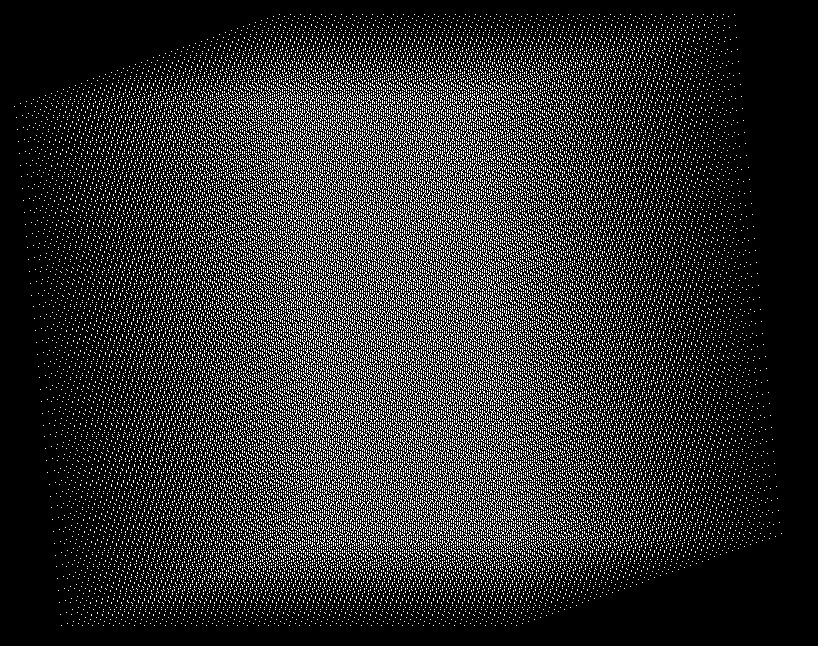
\includegraphics[width=\textwidth]{p91125.pdf}}
		\subcaption[]{91,125 particles (1700 fps)}
		\label{fig:p91125}
	\end{subfigure}
\hspace{-0.1in}
	\begin{subfigure}[b]{0.3\textwidth}
		{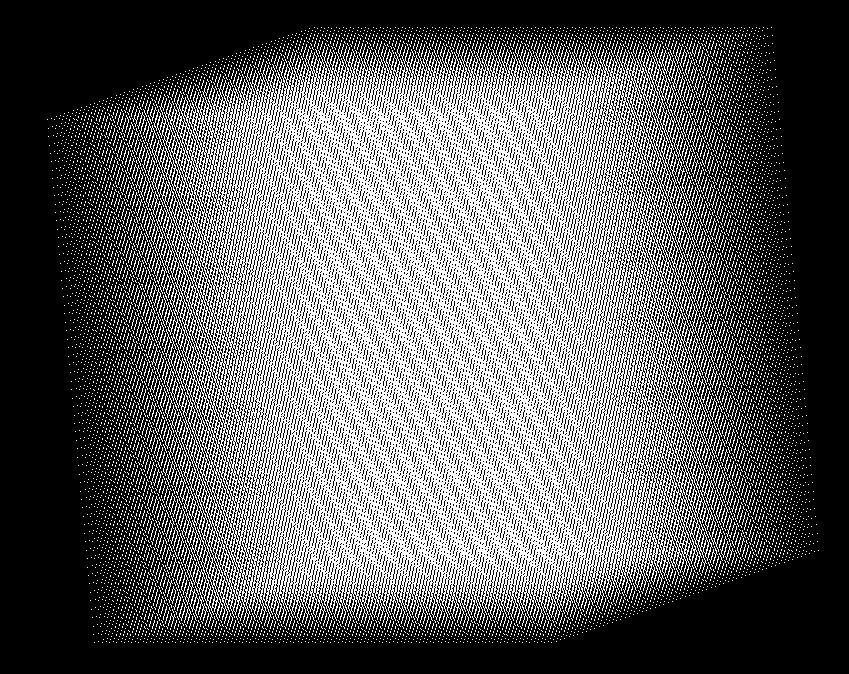
\includegraphics[width=\textwidth]{p250047.pdf}}
		\subcaption[]{250,047 particles (860 fps)}
		\label{fig:p250047}
	\end{subfigure}
\hspace{-0.1in}
	\begin{subfigure}[b]{0.3\textwidth}
		{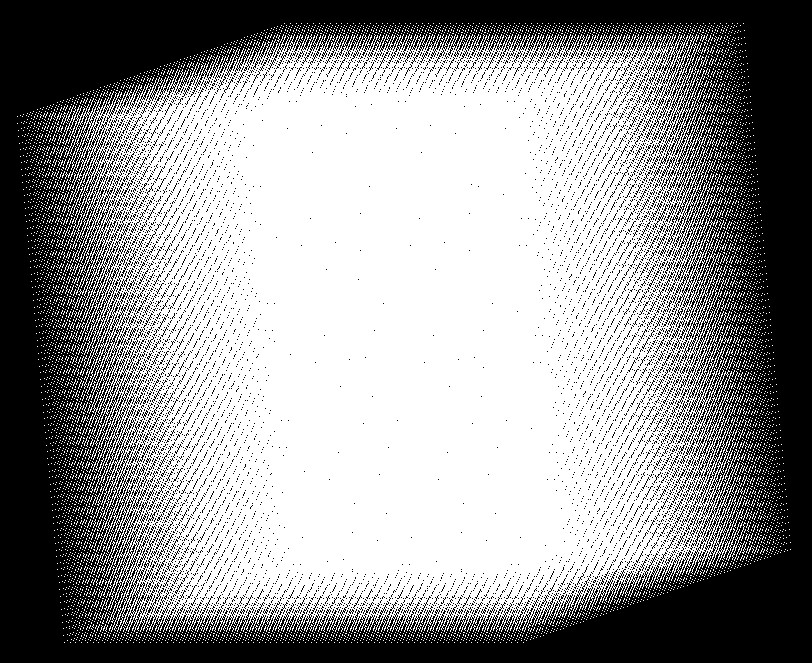
\includegraphics[width=\textwidth]{p531441.pdf}}
		\subcaption[]{531,441 particles (299 fps)}
		\label{fig:p531441}
	\end{subfigure}
\hspace{-0.1in}
	\begin{subfigure}[b]{0.3\textwidth}
		{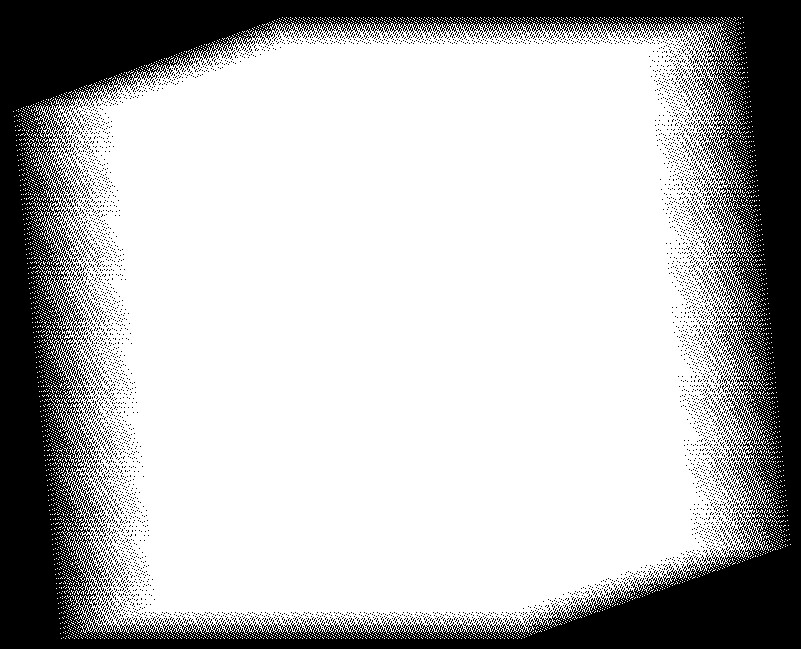
\includegraphics[width=\textwidth]{p1259712.pdf}}
		\subcaption[]{1,259,712 particles (130 fps)}
		\label{fig:p1259712}
	\end{subfigure}
\hspace{-0.1in}
	\begin{subfigure}[b]{0.3\textwidth}
		{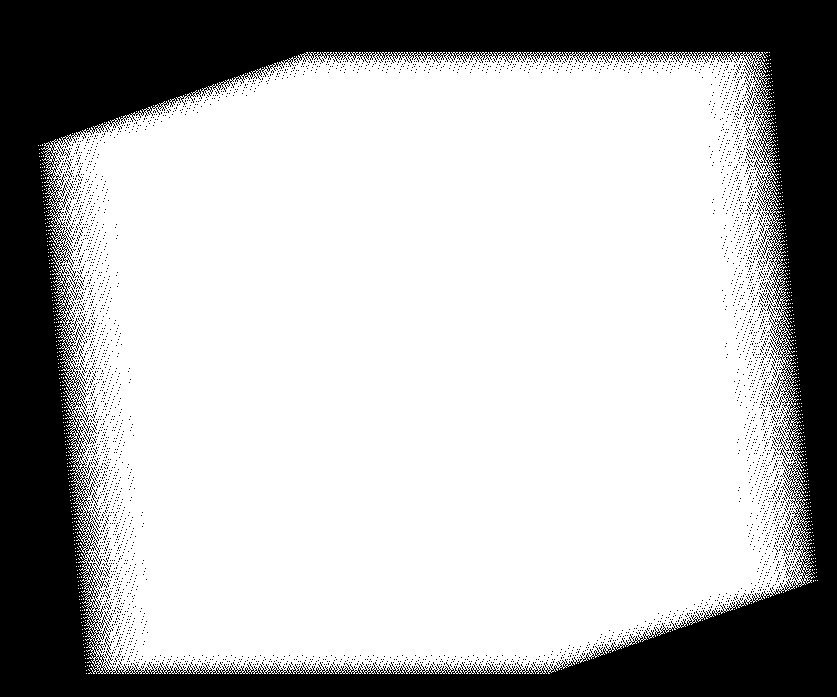
\includegraphics[width=\textwidth]{p2985984.pdf}}
		\subcaption[]{2,985,948 particles (48 fps)}
		\label{fig:p2985984}
	\end{subfigure}
\caption[TITLE:Cell Spans]{Frame captures illustrating particle
distributions at increasing densities with estimted frame rate. 
The examples shown were generated by maintaining a fixed (10x10x10) cell array
while increasing the number of particles occupying each cell. Similar
particle counts can also be achieved by increasing the size of the cell
array while maintaining a lower particle occupancy per cell. The latter
configuration is generally preferred because it reduces local cell
occupancy and therefore decreases the number of candidate interactions
evaluated during narrow-phase collision detection. This behavior aligns
well with the gPCD architecture, which benefits from distributing
particles across a larger number of cells rather than increasing the
number of particles contained within each cell.}

\label{fig:DensityGraphs}
\end{figure*}
\endgroup

Figure~\ref{fig:DensityGraphs} illustrates the increase in spatial
resolution achievable through increasing particle count. At 5,832
particles, the discrete nature of the particle representation remains
visually apparent. In contrast, the 2,985,984-particle configuration
approaches a visually continuous representation while retaining an
explicitly discrete particle formulation.

Despite this increase in particle density, the largest configuration
remains interactive, sustaining approximately 50 frames per second on
the evaluation platform. These results suggest that a single CPU-GPU
system can support particle-system scales traditionally associated with
high-performance computing resources.

The GPU-resident organization of the framework also facilitates
particle visualization and analysis. Because particle state remains
available within the graphics pipeline, quantities such as temperature,
velocity magnitude, and velocity direction can be mapped directly to
color during rendering with minimal additional computational cost. In
particular, HSV-based velocity-angle colorization provides an efficient
means of visualizing directional flow structures and other emergent
patterns in large-scale particle systems.
